
%hi
\documentclass{article}
\usepackage[margin=1in]{geometry} 
\usepackage{amsmath,amsthm,amssymb,amsfonts, fancyhdr, color, comment, graphicx, environ}
\usepackage{xcolor}
\usepackage{mdframed}
\usepackage[shortlabels]{enumitem}
\usepackage{indentfirst}
\usepackage{hyperref}
\usepackage{float}
\renewcommand{\footrulewidth}{0.8pt}
\hypersetup{
    colorlinks=true,
    linkcolor=blue,
    filecolor=magenta,      
    urlcolor=blue,
}


\pagestyle{fancy}



\newenvironment{problem}[2][Problem]
    { \begin{mdframed}[backgroundcolor=gray!20] \textbf{#1 #2} \\}
    {  \end{mdframed}}


\newenvironment{solution}{\textbf{Solution}}


\lhead{Kasra Amani}
\rhead{Real Time Systems} 
\chead{\textbf{Assignment 1}}
\lfoot{Sepideh Safari}
\rfoot{Sharif University of Technology}
\def\thesection{\alph{section}}

\begin{document}
\title{\Large Embedded Systems  \\[0.5cm]
        \bf\Large Assignment 1}
\author{\large Author: Kasra Amani\\ \normalsize Student No. 98101171 \\ \ \\}
\date{\large Date Last Edited: \today}

\makeatletter
    \begin{titlepage}
        \begin{center}
	   { 
\includegraphics[width=13cm]{sharif.png}}
	   {\ \\ \ \\}
        \vbox{}\vspace{5cm}
            {\@title }\\[3cm] 
            {\@author}
            {\large Instructor: \bf Prof. Ansari\\ \ \\}
            {\@date\\}

        \end{center}
    \end{titlepage}
\makeatother%not necessary but looks fancy
    \begin{problem}{1}
    	The Ariane flight V88 was a flight of the Ariane 5 space rocket that failed 43 seconds after launch due to the rocket self-destructing because it veered off its predestined flight path. This happened due to an error in the code.
    	\begin{figure}[H]
    	\centering
    	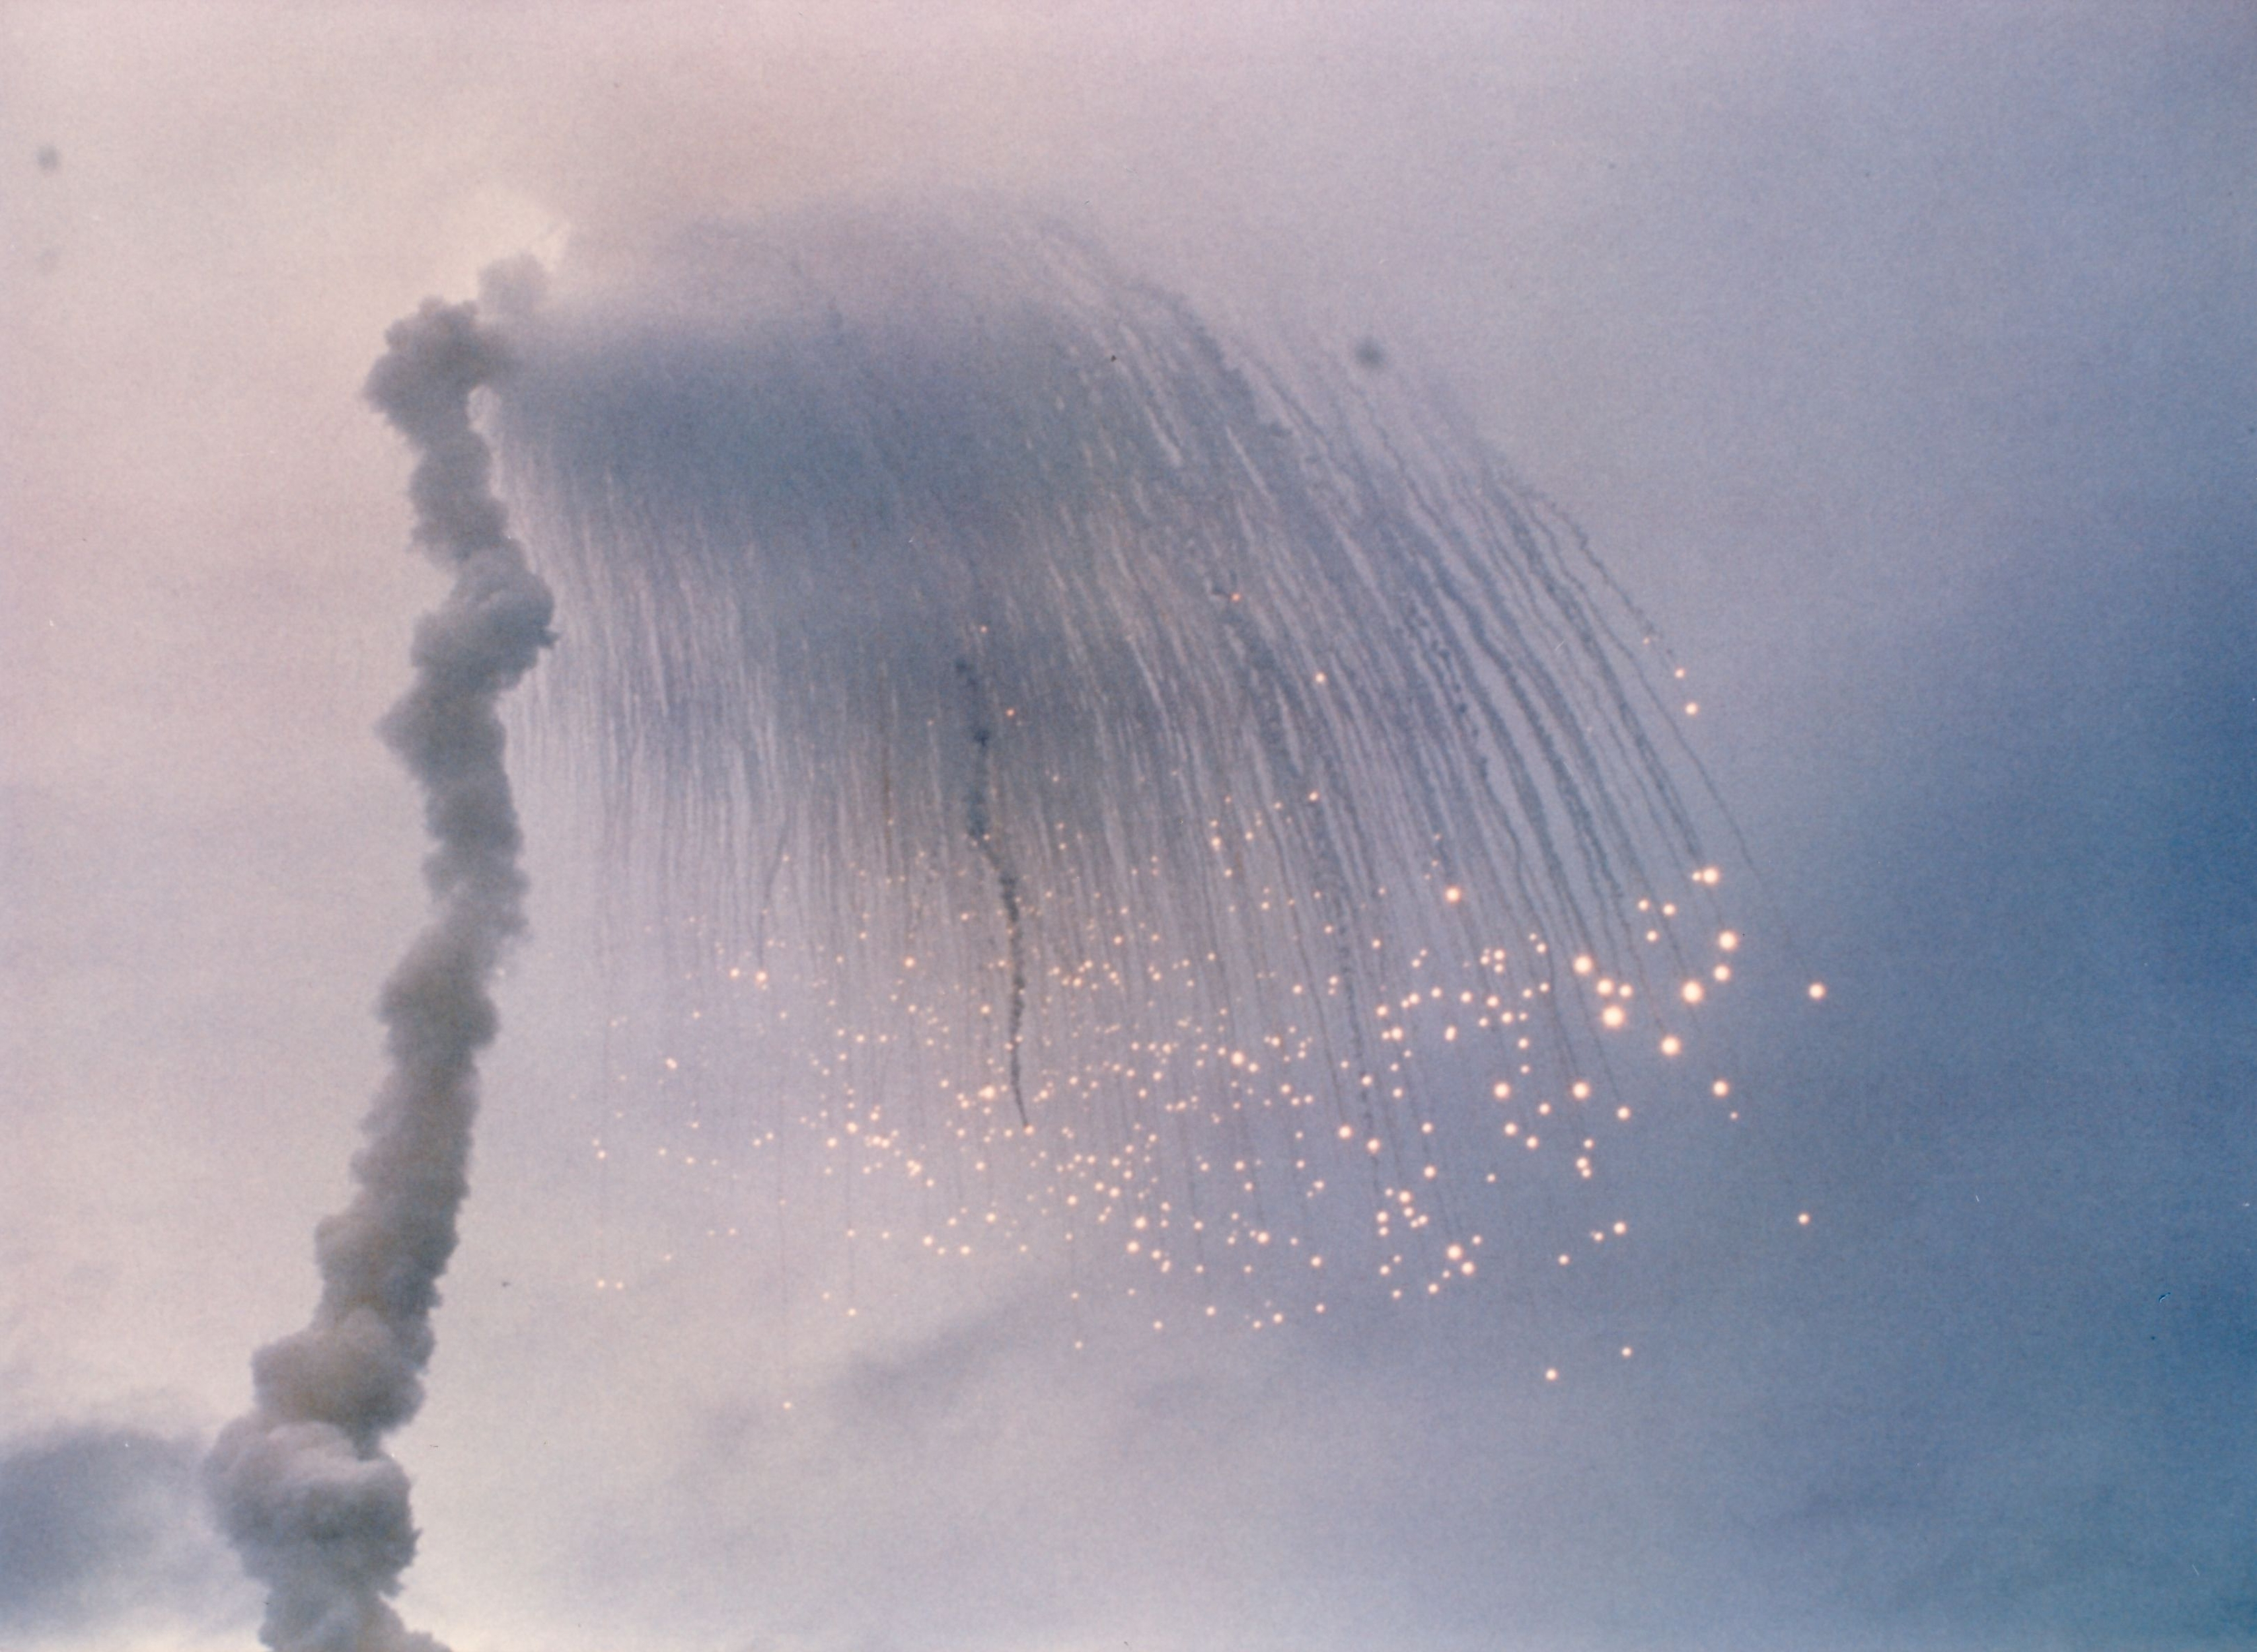
\includegraphics[width=1\linewidth]{ariane5.jpg}
    	\end{figure}
    \end{problem}
    
    \newpage
    \begin{problem}{2}
    	The Boeing 737MAX was an aircraft model designed by Boeing which experienced a series of crashes a few years ago; the problem (although not specifically mentioned by Boeing) seems to be in the MCAS (Maneuvering Characteristics Augmentation System) which upon takeoff, would assume that the aircraft was stalling (a phenomenon in which the plane does not have enough thrust to gain altitude and goes down) and automatically nosedives down. This is a great safety feature but the issue was the aircraft AI was doing this upon takeoff and the plane would crash into the ground.
    	\begin{figure}[H]
    	\centering
    	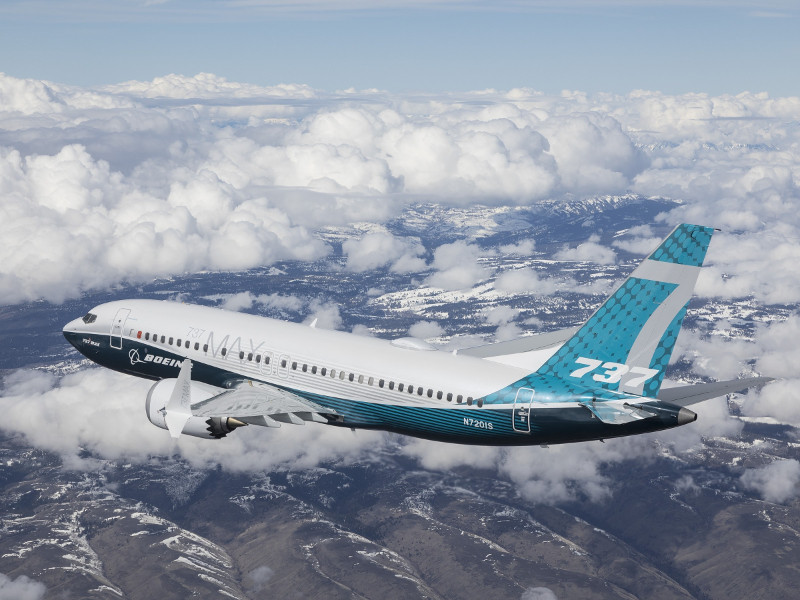
\includegraphics[width=1\linewidth]{737max.jpg}
    	\end{figure}
    \end{problem}


\end{document}